\documentclass[12pt]{article}
\usepackage[utf8]{inputenc}
\usepackage{listings}
\usepackage{xcolor}
\usepackage{geometry}
\usepackage{hyperref}
\usepackage{graphicx}

\graphicspath{ {media/} }

\geometry{a4paper, margin=1in}
\hypersetup{
    colorlinks=true,
    linkcolor=blue,
    filecolor=magenta,  
    urlcolor=cyan,
    pdftitle={Practice Session Report},
    pdfpagemode=FullScreen,
}

\lstset{
    language=Java,
    basicstyle=\ttfamily\footnotesize,
    keywordstyle=\color{blue}\bfseries,
    stringstyle=\color{red},
    commentstyle=\color{green},
    breaklines=true,
    numbers=left,
    numberstyle=\tiny\color{gray},
    frame=single,
    rulecolor=\color{black},
    showspaces=false,
    showstringspaces=false,
}

\renewcommand{\contentsname}{Table Of Contents}
\newcommand{\university}{\textit{\textbf{EST Safi}}}

\title{Java: Practice Session Report}
\author{Karim ELKHANOUFI}

\begin{document}

\maketitle

\newpage

\tableofcontents

\newpage

\section{Objective}
The objective of this practice session was to design and implement a
Java-based employee management system with a multi-layered architecture
including models, views, controllers, and database interactions.

\section{Assignment Overview}
The assignment involved creating the following components:
\begin{itemize}
    \item \textbf{Model}: A representation of employee data including
		attributes like name, email, phone, salary, post, and role.
    \item \textbf{DAO (Data Access Object)}: A layer to interact with the
		PostgreSQL database using SQL queries.
    \item \textbf{Controller}: Handles logic for adding, deleting, updating,
		and displaying employees.
    \item \textbf{View}: A graphical user interface (GUI) for user
		interactions.
\end{itemize}

\section{Code Implementation}

\subsection{Main Class}
\begin{lstlisting}
import Controllers.EmployeeController;
import DAO.EmployeeDAOImpl;
import Views.EmployeeView;

public class Main {
  public static void main(String[] args) {
    // Init the database connection
    EmployeeDAOImpl dao = new EmployeeDAOImpl();

    // Render the View
    EmployeeView ev = new EmployeeView();

    // Add controller for the view
    EmployeeController ec = new EmployeeController();
  }
}
\end{lstlisting}

\pagebreak

\subsection{DAO}
\subsubsection{DAO Interface}
\begin{lstlisting}
package DAO;

interface EmployeeDAOI {
  // Credentials
  public String url = "jdbc:postgresql://localhost:5432/java_db";
  public String dbuser = "postgres";   // Database user
  public String dbpw = "pg1234";       // Database password

  // Abstract methods
  public boolean addEmployee(Employee em);
  public boolean deleteEmployee(int id);
  public boolean updateEmployee(int id, Employee em);
}
\end{lstlisting}

\subsubsection{DAO Implementation}
\begin{lstlisting}
package DAO;

public class EmployeeDAOImpl implements EmployeeDAOI {
  // Constructor
  public EmployeeDAOImpl();
  
  // Methods to be override here
}
\end{lstlisting}

\pagebreak

\subsection{Model}
\begin{lstlisting}
package Models;

public class Employee {
  // Constructor
  public Employee(ResultSet rs);
  
  // Getters
  public int getId();
  public String getLname();
  public String getFname();
  public String getEmail();
  public double getSalary();
  public String getPhone();
  public String getPost();
  public String getRole();
  
  // Setters
  public void setId(int id);
  public void setLname(String lname);
  public void setFname(String fname);
  public void setEmail(String email);
  public void setSalary(double salary);
  public void setPhone(String phone);
  public void setPost(String post);
  public void setRole(String role);

  // methods for Controller intercations
  public boolean addEmployee();
  public static boolean deleteEmployee(int id);
  public boolean updateEmployee(int id);

  public String toString();
}
\end{lstlisting}

\subsection{Controller}
\begin{lstlisting}
package Controllers;

public class EmployeeController {
  // Constructor
  public EmployeeController();
  
  // Event listeners initialization methods
  private void initAddEvent();
  private void initDeleteEvent();
  private void initUpdateEvent();
  private void initShowEvent();
  
  // Useful View handling methods
  public static void populateTable();
  public static void emptyFields();
}
\end{lstlisting}

\subsection{View}
\begin{lstlisting}
package Views;

public class EmployeeView extends JFrame {
  // Constructor
  public EmployeeView();
}
\end{lstlisting}

\section{Results}
The application  was test in Ubuntu and PostgreSQL as a database management
system.

\begin{figure}[h]
  \centering
	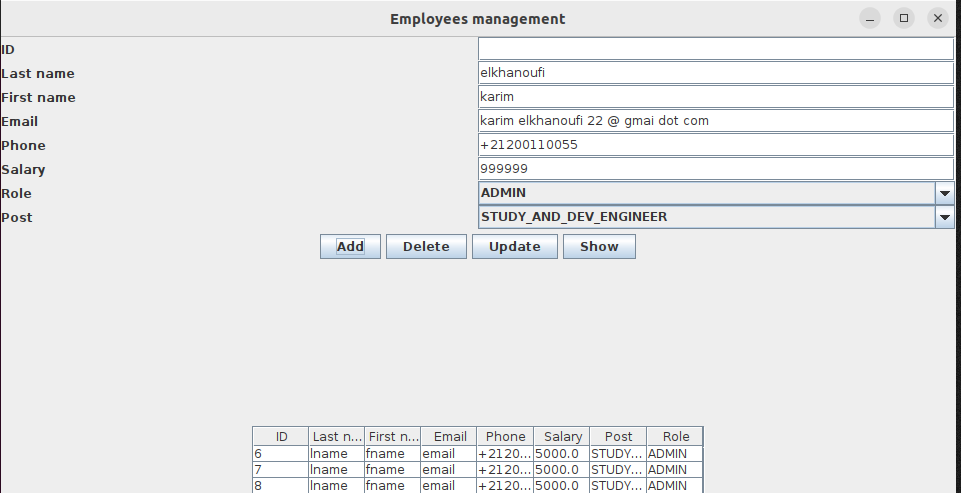
\includegraphics[width=0.5\textwidth]{preview.png}
  \caption{Application preview}
\end{figure}

The implementation successfully demonstrated the following functionalities:
\begin{itemize}
    \item Establishing a connection to a PostgreSQL database.
    \item Adding, deleting, and updating employee records through GUI
		interactions.
    \item Displaying employee data in a tabular format within the GUI.
\end{itemize}

\section{Challenges and Solutions}
\begin{itemize}
    \item \textbf{Challenge:} Handling SQL exceptions during database
		operations.
    \item \textbf{Solution:} Added try-catch blocks and proper error messages.
    \item \textbf{Challenge:} Synchronizing GUI updates with database changes.
    \item \textbf{Solution:} Implemented a method to repopulate the table
		dynamically after each operation.
\end{itemize}

\section{Conclusion}
The session provided hands-on experience in building a complete Java
application with GUI and database integration. This practice solidified
concepts of MVC architecture and SQL database interaction.

\section{References}
\begin{itemize}
    \item Java Documentation: \url{https://docs.oracle.com/en/java/}
    \item PostgreSQL documentaion: \url{https://www.postgresql.org/docs/}
    \item pgJDBC documentaion: \url{https://jdbc.postgresql.org/documentation/}
\end{itemize}

\end{document}
